\subsection{Bézier and B-splines functions}
Given the spline function now we have to define its shape. In literature, two main classes of functions are designed for KANs:
\begin{itemize}
    \item Bézier functions which consider all the domains but are complex to train \cite{bezier}
    \item B-splines functions which consider only a local domain but are easy to train \cite{kan_intro}.
\end{itemize}

The problem we are going to solve is that the spline function should pass through some tag points that will be adjusted during the training phase. To solve it let's consider a dual problem: imagine a character $C$ must pass through $n$ points $(P_1, \dots,P_n)$. The most obvious way to traverse them is to go straight from $P_i$ to $P_{i+1}$ but this movement does not appear natural because we desire a smooth traversal movement that can be described as $(n-1)$-degree polynomial as in Figure~\ref{fig:bezier}.  
\begin{figure}[H]
    \centering
    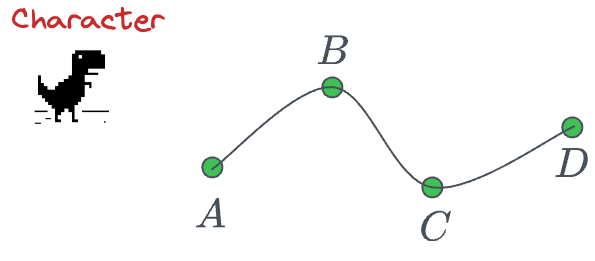
\includegraphics[width=0.5\linewidth]{Images/bezier.png}
    \caption{Example of 4-degree polynomial curve}
    \label{fig:bezier}
\end{figure}

The naive way to implement it is to define a function $h(x): \Re \to \Re$:

$$h(x) = a_{n-1}x^{n-1} + a_{n-2}x^{n-2} + \dots + a_1x +a_0 $$

then we can substitute points $(P_1, \dots,P_n)$ into the function $h$ and determine the values of the coefficients $(a_0, \dots,a_{n-1})$. Now we realize that we have to solve $N$ equations to determine the coefficients. Solving such a system of linear equations will be computationally expensive and almost infeasible for KANs. For this reason, we choose Bézier or B-splines functions.

\subsubsection{Bézier}
Bézier curves solve the problem more smartly. They provide a way to represent a smooth curve that passes near a set of control points without needing to solve a large system of equations as in Figure~\ref{fig:bezier2}.   
\begin{figure}[H]
    \centering
    \subfloat{%
        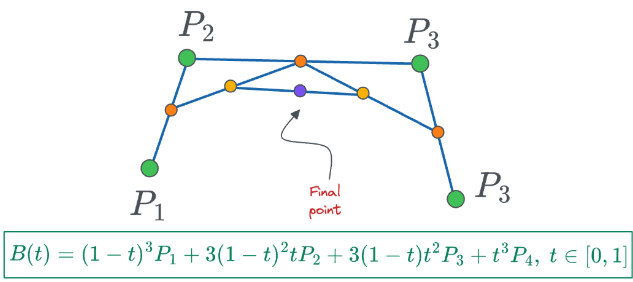
\includegraphics[width=0.55\linewidth]{Images/bezier2.png}%
        \label{fig:bezier2a}%
    }
    \hfill
    \subfloat{%
        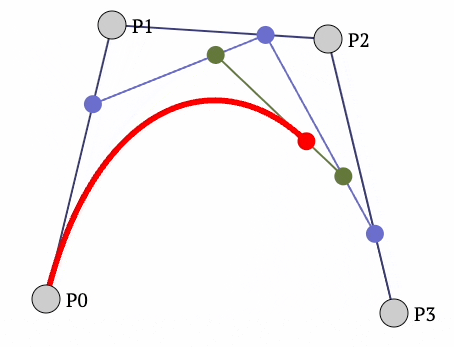
\includegraphics[width=0.30\linewidth]{Images/bezier3.png}%
        \label{fig:bezier2b}%
    }
    \caption{Example of 4-degree bezier curves}
    \label{fig:bezier2}
\end{figure}


We define the Bézier curve $b(t): \Re \to \Re$ noticing from low $n$ polynomials as in Figure~\ref{fig:bezier2} that the coefficients match with the binomial coefficients of $(1+t)^n$. Then we can derive the binomial definition of the Bézier curve as:

\[
\mathbf{b}(t) = \sum_{i=0}^n \binom{n}{i} (1-t)^{n-i} t^i \mathbf{P}_i, \quad t \in [0, 1]
\]

However, the problem is still the same as before. Having $N$ data points will result in a polynomial of degree $N-1$, which will be computationally expensive.

\subsubsection{B-splines}
B-splines provide a more efficient way to represent curves, especially when we deal with a large number of data. Unlike high-degree polynomials, B-splines use a series of lower-degree polynomial segments, which are connected smoothly.
In other words, instead of extending Bézier curves to tens of hundreds of data points, which leads to an equally high degree of the polynomial, we use multiple lower-degree polynomials and connect them to form a smooth curve as in Figure~\ref{fig:bezier4}.

\begin{figure}[H]
    \centering
    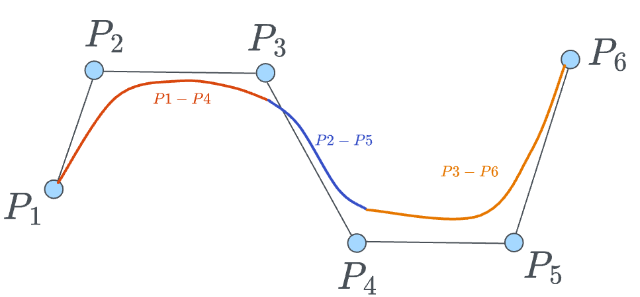
\includegraphics[width=0.5\linewidth]{Images/bezier4.png}
    \caption{Example of 6-degree B-spline curve}
    \label{fig:bezier4}
\end{figure}

When we have $n$ control points and we create $k$ degree polynomial Bézier curves, we get $(n-k)$ Bézier curves in the final Bsplines. We ensure also a certain continuity condition at the points where the curves meet:
\begin{itemize}
    \item Position Continuity: $C^0$ Continuity 
    \item Tangent Continuity: $C^1$ Continuity  
    \item Curvature Continuity: $C^2$ Continuity 
\end{itemize}

Similar to Bézier curves, we define the B-spline curve \( B(x): \Re \to \Re \) as a linear combination of the learnable position of points \( P_i \) and their associated non-learnable basis functions \( N_{i,k} \):


\[
\mathbf{B_i}(x) = \sum_{i=0}^n P_i N_{i,k} \Rightarrow \textbf{splines}(x ) = \sum_{i=0}^k c_i B_{i}(x) = \sum_{i=0}^k c_i \sum_{i=0}^n P_i N_{i,k}
\]

Finally, we have defined spline as a B-spline function linear combination. This is best choice for KANs, even though they consider only a local domain, because their strength lies in their easy trainability, even as the number of points increases.
